\documentclass{beamer}
\usepackage[utf8]{inputenc}
\usepackage{xspace}
\usepackage{xurl}
\usepackage{caption}
\usepackage{appendixnumberbeamer}
\usepackage{amsmath,amssymb}
\usepackage{dsfont}
\usepackage{verbatim}
\usepackage{bigints}
\usepackage{tikz}
\usepackage{mathrsfs}
\DeclareMathOperator{\EX}{\mathbb{E}}%
\newcommand{\Prob}{\text{I\kern-0.15em P}}
\usepackage{dsfont}
%\newcommand{\1}[1]{\mathds{1}\left[#1\right]}


\let\OldTextgreater\textgreater
\renewcommand{\textgreater}{\OldTextgreater\xspace}%
\setbeamertemplate{itemize subitem}{$\rightarrow$}

\usetheme{Madrid}
\useoutertheme[subsection=false]{miniframes} % Alternatively: miniframes, infolines, split
\useinnertheme{circles}
\definecolor{UBCgrey}{RGB}{51, 51, 178} % UBC Blue (primary)
\definecolor{UBCblue}{RGB}{38, 38, 134} % UBC Grey (secondary)
\setbeamercolor{palette primary}{bg=UBCblue,fg=white}
\setbeamercolor{palette secondary}{bg=UBCblue,fg=white}
\setbeamercolor{palette tertiary}{bg=UBCblue,fg=white}
\setbeamercolor{palette quaternary}{bg=UBCblue,fg=white}
\setbeamercolor{structure}{fg=UBCblue} % itemize, enumerate, etc
\setbeamercolor{section in toc}{fg=UBCblue} % TOC sections
% Override palette coloring with secondary
\setbeamercolor{subsection in head/foot}{bg=UBCgrey,fg=white}

\graphicspath{ {./images/} }

%------------------------------------------------------------
\title[To Reload or Not To Reload?] %optional
{To Reload or Not To Reload? \\ Motivating Risk-Averse Executives Using Employee Stock Options With An Enhanced Reload Feature}

\subtitle{}

\author[Djekic D.] % (optional)
{Djekic Davor \ \inst{1}}

\institute[] % (optional)
{
  \inst{1}%
  %Department of Economics\\
  Bocconi University
}

\date[July 2024] % (optional)
{July 17/18, 2024}

%\logo{\includegraphics[height=0.7cm]{bocconi_logo.png}}

%End of title page configuration block
%------------------------------------------------------------

%------------------------------------------------------------


\begin{document}

%The next statement creates the title page.
\frame{\titlepage}

%---------------------------------------------------------


\frame{\tableofcontents}


\section{Employee Stock Options}
\begin{frame}{Employee Stock Options}
    \begin{itemize}
        \item ESOs are call options on firm’s stock $\rightarrow$ $\pi \uparrow$ when stock appreciates
        \item Features: strike price, maturity, vesting, OTM/ATM/ITM  +  non-transferability, limited hedging
        \item Why? Incentive alignment, talent attraction, deferred cash expenditure, \dots
        \item Value = Intrinsic value + Time value 
    \end{itemize}

    \vspace{10pt}
    \begin{figure}[!h]
        \centering
        \begin{tikzpicture}
            % Draw horizontal line
            %\draw (3,0) -- (13,0);
            
            % Draw ticks
            \draw (3,-0.1) -- (3,0.1) node[anchor=south] {};
            \draw (5,-0.1) -- (5,0.1) node[anchor=south] {};
            \draw (13,-0.1) -- (13,0.1) node[anchor=south] {};
            
            % Add labels
            \node at (3,-0.3) {t=0};
            \node at (5,-0.3) {t=2};
            \node at (13,-0.3) {t=10};
            
            % Draw colored lines and labels
            \draw[red densely dotted] (3,0) -- node[above] {nonvested} (5,0);
            \draw[blue] (5,0) -- node[above, yshift=1.5pt] {vested} (13,0);
        \end{tikzpicture}
    \end{figure}
    
    \note[item]{Employee (or Executive) Stock Options are compensation contracts granted from an em- ployer to its executives. They entitle the holder to buy a certain number of shares of the company’s stock at a predetermined price (the strike price) within a certain timeframe (the maturity), usually starting from a certain date (the vesting date). The holder is not however obliged to exercise the option, and will do so when it gives her positive utility (i.e., when the stock price is above the strike price). Together with cash and other benefits (e.g., restricted stock, performance bonuses), they form the compensation package of an executive. They usually come with some other features, such as non-transferability — the holder cannot sell them as would usually do with traditional options — and restrictions on short-selling the underlying stock, which limit the possibility of hedging the option.}
    \note[item]{Ability to attract and retain talent, especially motivated and entrepreneurial employees (Hall and Murphy, 2003).}
    \note[item]{We say that an option is in-the-money (ITM) when the stock price is above the strike price, out-of-money (OTM) when the stock price is below the strike price, and at-the-money (ATM) when the stock price is equal to the strike price.}
    \note[item]{The difference between the stock price and the strike price is called the intrinsic value of the option, while the difference between the option price and the intrinsic value is called the time value of the option}
\end{frame}


\section{Literature Review}
\begin{frame}{Literature Review I}
    \begin{itemize}
        \item Sharp increase starting in 1990: ownership concentration, liquidity, CEO and institutional ownership, investment intensity, and historical market returns \textit{(Pasternack et al., 2002)}
        \item Now, in US: 6,533 ESO plans, holding total assets \$2.1+ trillion \textit{(NCEO, 2024)}; but preference towards other performance-based compensation \textit{(Frydman and Jenter, 2010)}
        \item Separation corporate ownership and control (\dots) $\rightarrow$ Re-align incentives \textit{(Jensen and Meckling, 1976)} + take higher risk \textit{(Jensen and Murphy, 1990)}
        \item Undiversified managers at avg NYSE firm value ESOs 30\% less than market value, while those at startups value theirs 47\% less \textit{(Meulbroek, 2001)} $\rightarrow$ Deadweight loss
    \end{itemize}

    \note[item]{The misalignment between the two started with the separation of corporate ownership and corporate control at the beginning of the past century, which led to the need for a direct link between executive’s realized compensation and the firm’s performance. Indeed, the shareholders capture most of the benefits while the employees bear most of the costs, and thus the need to link the employee’s compensation to some performance measure, for example the stock price in the case of publicly traded firms.}
    \note[item]{Hall and Murphy (2002) present the divergence between firm cost and executive value, arguing that the former is the value if the firm were to sell the tradable and hedgeable option to an outside investor, while the latter is the value for the executive, who is not able to hedge the option and is exposed to the total risk of the firm.}
\end{frame}

\begin{frame}{Literature Review II}
    \begin{itemize}
        \item Executives' risk aversion is lower than average, but still there are some differences - also related to age and gender (Brenner (2015); Carter, Franco, and Gine (2017); Iqbal, Sewon, and Baek (2006))
        \item \textit{Cook, 1987} introduces reload options: at exercise, receive one stock and one new option
        \item \textit{Huand et al. (2013)} introduce Dynamic ESOs: at exercise, receive part in stock and part in option 
        \begin{itemize}
            \item $\rightarrow$ Recoup time value
            \item $+$ For executive: lock-in gain, decrease risk exposure, better compensation
            \item $+$ For firm: higher risk-taking, tax benefits
        \end{itemize}
    \end{itemize}
    \note[item]{Time value gets recouped by allowing the executive to still be exposed to possible stock appreciation + optionality of exercise.}
    \note[item]{Another advantage of reload options is that the exercise does not change the manager’s total equity holding but only its composition, which ties the executive to the firm’s longer-term performance and is thus a desirable feature from an incentive perspective + encourages stock ownership}
    \note[item]{The exercise policy of American options prescribes indeed that a risk-neutral agent would not exercise earlier, if not for receiving some additional benefits of possessing the stock (e.g., dividends, voting rights, etc.).}
\end{frame}


\section{The Problem}
\begin{frame}{The Problem}
    2 facts:
    \begin{enumerate}
        \item Risk aversion (+ non-transferability) drives the difference between executive valuation and market value of ESOs
        \item Executives are exposed to undiversified (firm-specific) risk
    \end{enumerate}
    \vspace*{10pt}
    $\rightarrow$ \textbf{Idea: Can we re-align values and incentives by offering two different options, one of which offers a risk premium?}
    \begin{itemize}
        \item Give the \textit{right} option to the \textit{right} executive
        \item Who gets what?
        \item Who is better off in the equilibrium?
    \end{itemize}
\end{frame}


\section{Theoretical Model}
\begin{frame}{Theoretical Model}
    \framesubtitle{Main Elements}
    \begin{enumerate}
        \item Stock Price
        \item 2 Options: RN and $R_{\alpha, \gamma}$
        \item Risk-averse executives with heterogeneous risk aversion
        \item Public, risk-neutral firm
        \item Problem with adverse selection and moral hazard
    \end{enumerate}
\end{frame}

\begin{frame}{Theoretical Model}
    \framesubtitle{Stock Price}
    \begin{itemize}
        \item Geometric Brownian motion process $W = \{ W_t, \mathscr{F}_t \}_{t \ge 0}$ on a probability space $(\Omega, \mathscr{F}, P)$
        \item Stock price follows: $dS_t = \mu S_t dt + \bar{\sigma} S_t dW_t$
        \vspace*{5pt}
        \item When managed by the executive: $dS_t = \alpha a_t dt + \delta \sigma_t S_t dt + \bar{\sigma} S_t dW_t$
        \begin{itemize}
            \item $a = \{a_t\}_{t \ge 0}$ is effort and $\sigma = \{\sigma_t\}_{t \ge 0}$ is volatility
            \item $\delta \in [0,1]$: impact of project on firm's volatility
            \item $\alpha \in [0,1]$: relevance of executive
        \end{itemize}
    \end{itemize}
    \note[item]{A standard geometric Brownian motion process $W = \{ W_t, \mathscr{F}_t \}_{t \ge 0}$ on a probability space $(\Omega, \mathscr{F}, P)$ drives the stock price. }
\end{frame}

\begin{frame}{Theoretical Model}
    \framesubtitle{2 Options: $RN$ and $R_{\alpha, \gamma}$}
    \begin{itemize}
        \item Fix $S_0, K, T, v \rightarrow$ $RN$ + $R_{\alpha, \gamma}$ for $\alpha, \gamma \in [0,1]$ 
        \item $R_{\alpha, \gamma}$: at exercise, (i) $\alpha$ in stock, (ii) $(1 - \alpha + \gamma)$ in new RN
        \begin{itemize}
            \item $\gamma > 0$: risk premium
            \item $R_{1,0}$ = $RN$
        \end{itemize}
        \item Contract space is $\Theta = \Bigl( \mathds{1}_{RN}, \bigl\{ \mathds{1}_{R_{\alpha, \gamma}} \bigr\}_{\alpha \in (0,1), \gamma \in [0, 1)} \Bigr) \times \mathbb{Z}^+ $
        \begin{itemize}
            \item $\rightarrow \theta_{RN} = (\mathds{1}_{RN}, n)$ and $\theta_{R} = (\mathds{1}_{R_{\alpha, \gamma}}, n)$, with $n$ fixed
        \end{itemize}
    \end{itemize}
\end{frame}

\begin{frame}{Theoretical Model}
    \framesubtitle{2 Options: $RN$ and $R_{\alpha, \gamma}$}
    %DRAW R option (0.75, 0.1)
    %0, t_v, \tau, t_v, T+\tau; \alpha, \gamma

    %Role of vesting period + why it is risky

\end{frame}



\begin{frame}{Theoretical Model}
    \framesubtitle{Risk-averse executives}
    \begin{itemize}
        \item $\rho \in \{\rho_L, \rho_H\}$ s.t. $\rho_L < \rho_H$  
        \begin{itemize}
            \item $\lambda = \Prob(\rho = \rho_L)$ is common knowledge
        \end{itemize}
        \item $ W_t = n_S S_t + n_O (S_t-K)^+ + c(1+r_f)^t   $
        \begin{itemize}
            \item $W_0$ determines the composition of portfolio: $50-50$ or $67-33$ 
        \end{itemize}
        \item $ \bar{u}(W_t) = \frac{W_t^{1-\rho}}{1-\rho} $
        \item $ u_\rho (W_t, a_t) = \frac{W_t^{1-\rho}}{1-\rho} - \frac{1}{2}a_t^2 $
        \item $ \rightarrow U_\rho (a, \sigma) = \EX \Biggl[r \int_{0}^{T} e^{-rt} u_\rho (W_t, a_t) dt \Biggr]$
        \item \textbf{Chooses $(a, \sigma, \theta) \in \{a_L, a_H\} \times \{\sigma_L, \sigma_H\} \times \{\theta_{RN}, \theta_{R_{\alpha, \gamma}} \} $}
    \end{itemize}
    \note[item]{Coles, Daniel, and Naveen (2006) argues this effect may not be linear, as the inclusion of more and more performance-based and equity- based compensation in the executive’s pay package has led to a higher sensitivity of the executive’s wealth to the stock price, which in turn has led to a higher risk-taking behavior by the executive.}
    \note[item]{Note that choice of volatility is NOT (directly, at least) costly.}
    \note[item]{Clearly, denoting the $\rho_L$ type as risk-lover does not mean she always prefers to be exposed to more risk rather than less, but simply that she is less risk averse than the other type. }
\end{frame}

\begin{frame}{Theoretical Model}
    \framesubtitle{Public, risk-neutral firm}
    \begin{itemize}
        \item $ \Pi (\alpha, \gamma; \beta, \mu) = \beta \EX \Big[ S_T \Big] - \Big[ \mu C(\theta_{RN}) + (1-\mu) C(\theta_{R_{\alpha, \gamma}}) \Big]$ 
        \begin{itemize}
            \item In principle, $\mu \ne \lambda$
        \end{itemize}
        \item \textbf{Chooses $(\alpha, \gamma)$ for $R_{\alpha, \gamma}$}
    \end{itemize}
    \note[item]{$\beta$ measures how relevant it is for the firm to maximize the stock price at time T --- e.g., firms with large capitalization may have higher betas}
\end{frame}

\begin{frame}{Theoretical Model}
    \framesubtitle{Agent's Problem}

    \begin{equation*}
        \begin{aligned}
        \max_{a, \sigma, \theta} \quad & U_\rho (a, \sigma, \theta) \\
        \textrm{s.t.}       \quad & a \in \{ a_L, a_H \} \\
                            \quad & \sigma \in \{ \sigma_L, \sigma_H \} \\
                            \quad & \theta \in \{\theta_{RN}, \theta_{R_{\alpha, \gamma}} \} \\
                            \quad & U_\rho(a, \sigma, \theta) \ge \hat{U}  \\
        \end{aligned}
    \end{equation*}
\end{frame}

\begin{frame}{Theoretical Model}
    \framesubtitle{Firm's Problem(s)}
    
    \begin{equation*}
        \begin{alignedat}{2}
            \max_{\alpha, \gamma} \quad & \Pi (\alpha, \gamma; \beta, \mu) \\
            \textrm{s.t.}       \quad & U_{\rho}(a^*, \sigma^*, \theta^*) \ge \hat{U} & \quad & \forall \rho \in \{ \rho_L, \rho_H \}\\
                                \quad & U_{\rho}(a^*, \sigma^*, \theta^*) \ge U_{\rho}(a, \sigma, \theta) &\quad& \forall \rho \in \{ \rho_L, \rho_H \}\\
                                \quad & &\quad& \forall a \in \{ a_L, a_H \}, \\
                                \quad & &\quad& \forall \sigma \in \{ \sigma_L, \sigma_H \}, \\
                                \quad & &\quad& \forall \theta \in \{ \theta_{RN}, \theta_{R_{\alpha, \gamma}} \} \\ 
        \end{alignedat}
    \end{equation*}

\end{frame}


\section{Two Approaches}
\begin{frame}{Two Approaches}
    \begin{columns}[c]
        \begin{column}{0.5\textwidth} 
            \centering
            \Huge \textbf{1}\\
            \large
            \textbf{Qualitative Analysis}\\
            \normalsize
            \vspace*{5pt}
            Valuation of Options\\
            Analysis of incentives: Delta + Vega
        \end{column}
        \begin{column}{0.5\textwidth}
            \centering
            \Huge \textbf{2}\\
            \large
            \textbf{Numerical Simulations}\\
            \normalsize
            \vspace*{5pt}
            Parameter Choice\\
            Simulations' results
        \end{column}
    \end{columns}
\end{frame}


\subsection{Qualitative Analysis}
\begin{frame}{1. Qualitative Analysis}
    \framesubtitle{Valuation of Options}

    \begin{itemize}
        \item For Firm: binomial (risk-neutral) pricing
        \begin{itemize}
            \item C($RN$) and C($R_{\alpha, \gamma}$) computed backwards, with early exercise multiple technique by \textit{Hull and White (2004)}
            \item $R_{\alpha, \gamma}$ valuation accounts for recouped time value
        \end{itemize}
        \item For Executive: utility maximization
        \begin{itemize}
            \item $E_c$ such that $U_\rho(n_s, n_o, c) = U_\rho(n_S, 0, c + E_c)$
        \end{itemize} 
        \vspace*{5pt}
        \item $\rightarrow$ $R_{\alpha, \gamma}$ is always more expensive than $RN$, increasingly in $\alpha$ and $\gamma$
        \item $\rightarrow$ Executive value is always lower than firm value, but more stable for 50-50 agent
        \begin{itemize}
            \item May be slightly estimated because utility-based method does not predict early exercise \textit{Grasselli and Henderson (2009)}
        \end{itemize}
    \end{itemize}
    \note[item]{rn_eso is lower bound for r_eso, bc the latter has also non-negative time value.}
    \note[item]{Note that the value of adding $\gamma$ is two-fold: first, as a proper exercise compensation since the executive gets stock and options worth $(1+\gamma)$ the number of options she previously held, and second as time value recovered. Therefore, we propose the valuation methodology in snippet \ref*{fig:val_r} for our R option which embeds this double edge provided by $\gamma$: \verb|1+gamma*(S - K)| captures the first effect, \verb|(1-alpha+gamma)*(black_scholes(S,K,T,r,sigma)-(S-K))| the second.}
\end{frame}

\begin{frame}{1. Qualitative Analysis}
    \framesubtitle{Binomial tree with $n=2$}
    \begin{figure}[!h]
        \vspace*{10pt}
        \centering
        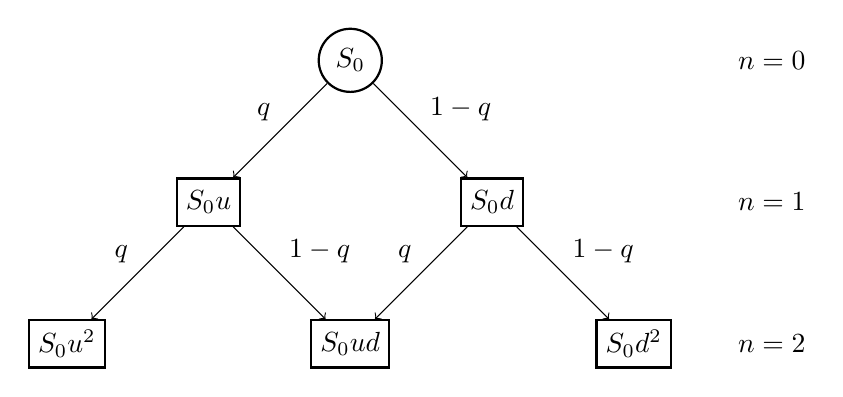
\begin{tikzpicture}[
            roundnode/.style={circle, draw=black, thick, minimum size=6mm},
            squarednode/.style={rectangle, draw=black, thick, minimum size=6mm},
            scale=1.2
          ]
          
          %Nodes
          \node[roundnode] at (0,0) (A) {$S_0$};
          \node[squarednode] at (-1.5,-1.5) (B) {$S_0 u$};
          \node[squarednode] at (1.5,-1.5) (C) {$S_0 d$};
          \node[squarednode] at (-3,-3) (D) {$S_0 u^2$};
          \node[squarednode] at (0,-3) (E) {$S_0 ud$};
          \node[squarednode] at (3,-3) (F) {$S_0 d^2$};  
          
          %Lines
          \draw[->] (A) -- (B) node[midway,above left] {$q$};
          \draw[->] (A) -- (C) node[midway,above right] {$1-q$};
          \draw[->] (B) -- (D) node[midway,above left] {$q$};
          \draw[->] (B) -- (E) node[midway,above right] {$1-q$};
          \draw[->] (C) -- (E) node[midway,above left] {$q$};
          \draw[->] (C) -- (F) node[midway,above right] {$1-q$};
          
          %Labels
          \node[right] at (4,0) {$n=0$};
          \node[right] at (4,-1.5) {$n=1$};
          \node[right] at (4,-3) {$n=2$};
        
        \end{tikzpicture}
        %\caption{Representation of the binomial tree with n=2} 
    \end{figure}
\end{frame}


\begin{frame}{1. Qualitative Analysis}
    \framesubtitle{Incentives}

    \begin{itemize}
        \item Delta and vega are sensitivities of the option price to stock price and volatility 
        \begin{itemize}
            \item \textbf{Objective:} predicted, by firm
            \item \textbf{Subjective:} actual, by executive 
        \end{itemize}
        \item Computations are limited by computing power (6-8h to run one simulation)
    \end{itemize}
\end{frame}

\begin{frame}{1. Qualitative Analysis}
    \framesubtitle{Effort Incentives}

    \begin{columns}[c]
        \begin{column}{0.5\textwidth} 
            \centering
            RN option \\
            \begin{figure}[!h]
                \centering
                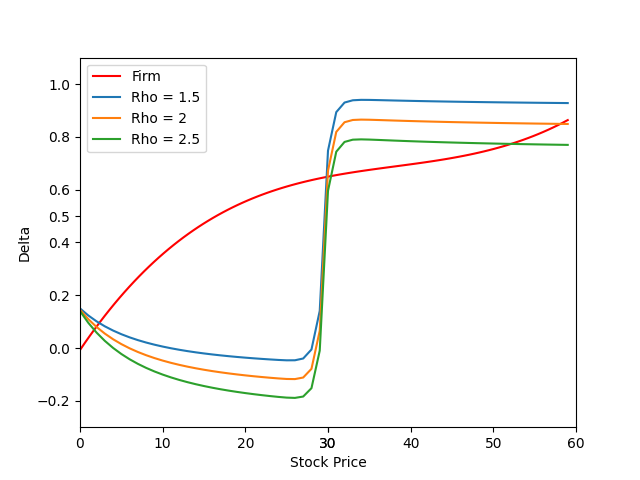
\includegraphics[width=\textwidth]{../fig/4/delta_comp.png}
            \end{figure}
        \end{column}
        \begin{column}{0.5\textwidth}
            \centering
            $R_{0.75, 0.1}$ for $\rho = 2$ executive \\
            \begin{figure}[!h]
                \centering
                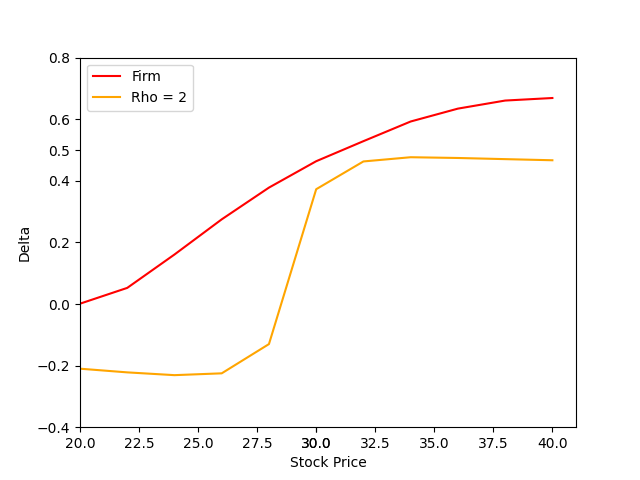
\includegraphics[width=\textwidth]{../fig/4/r_delta_comp.png}
            \end{figure}
        \end{column}
    \end{columns}
\end{frame}

\begin{frame}{1. Qualitative Analysis}
    \framesubtitle{Volatility Incentives}

    \begin{columns}[c]
        \begin{column}{0.5\textwidth} 
            \centering
            RN option
            \begin{figure}[!h]
                \centering
                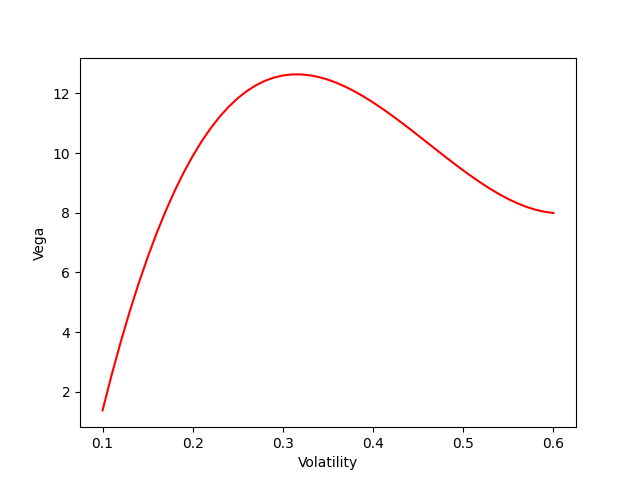
\includegraphics[width=0.5\textwidth]{../fig/4/vega_obj.png}
            \end{figure}
            \begin{figure}[!h]
                \centering
                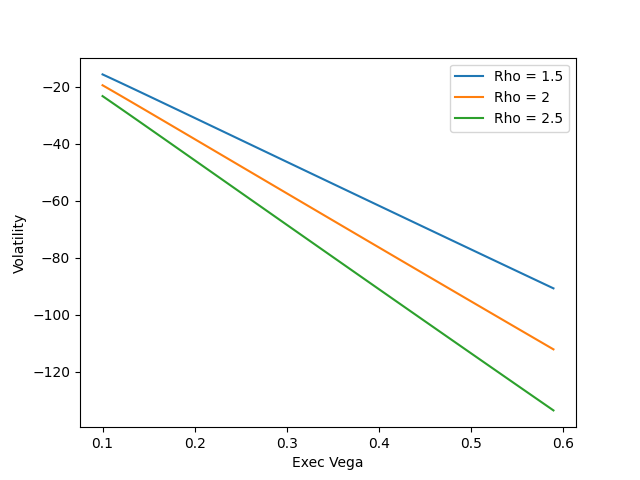
\includegraphics[width=0.5\textwidth]{../fig/4/vega_subj.png}
            \end{figure}
        \end{column}
        \begin{column}{0.5\textwidth}
            \centering
            $R_{0.75, 0.1}$ for $\rho = 2$ executive
            \begin{figure}[!h]
                \centering
                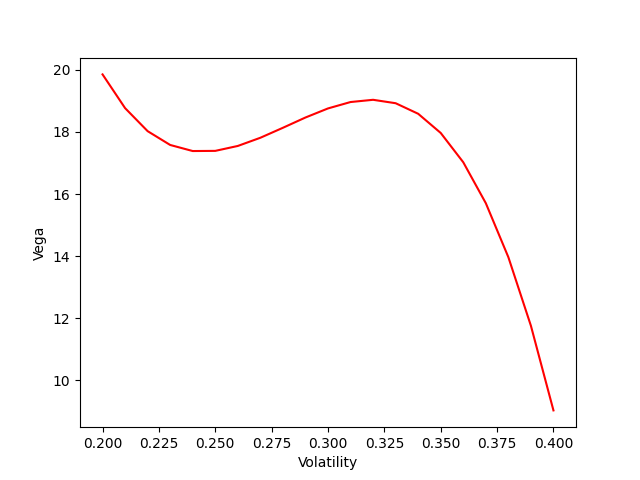
\includegraphics[width=0.5\textwidth]{../fig/4/r_vega_obj.png}
            \end{figure}
            \begin{figure}[!h]
                \centering
                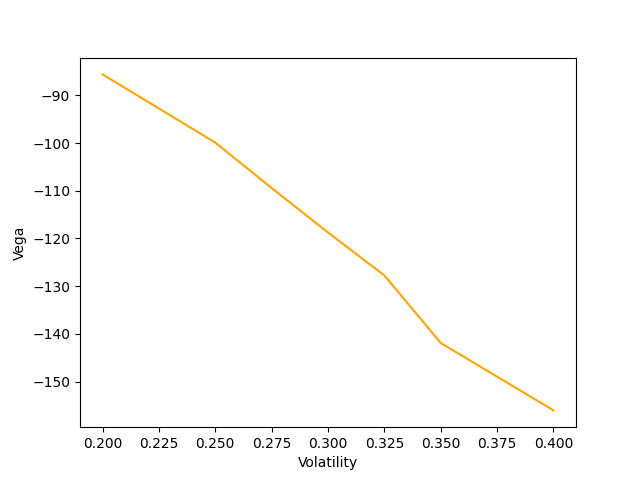
\includegraphics[width=0.5\textwidth]{../fig/4/r_vega_subj.png}
            \end{figure}
        \end{column}
    \end{columns}
\end{frame}


\begin{frame}{1. Qualitative Analysis}
    \framesubtitle{Incentives}

    \begin{itemize}
        \item Delta and vega are sensitivities of the option price to stock price and volatility 
        \begin{itemize}
            \item \textbf{Objective:} predicted, by firm
            \item \textbf{Subjective:} actual, by executive 
        \end{itemize}
        \item Computations are limited by computing power (6-8h to run one simulation)
        \item $\rightarrow$ Objective incentive is always higher than subjective incentive, except for effort incentive with RN option slightly OTM/ITM
        \item $\rightarrow$ Incentives under the $R_{\alpha, \gamma}$ option are always lower than under the RN option
    \end{itemize}
\end{frame}

\subsection{Numerical Simulations}
\begin{frame}{Numerical Simulations}
    \begin{itemize}
        \item We run 100 paths, each with 5,000 points (one per trading day)
        \item Stock price simulations $\rightarrow$ Agent's controls $\rightarrow$ Firm's choice
        \item \textbf{Assume constant effort and volatility $\rightarrow$ NO instantaneous incentives}
        \item We set T=20 years; $\rho_L = 1.5$, $\rho_H = 2.5$ (Carpenter, 1998); $y_{R1} = 6$, $y_{RN} = y_{R2} = 7$ (Murphy and Vance (2019) for RN) $a_L = 0$, $a_H = 1$, $\sigma_L = 0$, $\sigma_H = 0.01$
        \item We allow for $\alpha \in A = \{0.2, 0.5, 0.6, 0.7, 0.75, 0.8, 0.9, 1\}$ and $\gamma \in \Gamma = \{0, 0.05, 0.1, 0.15, 0.2, 0.25, 0.5, 0.75, 1\}$
        \item Principal ranks all $(\alpha, \gamma, a^*_{\rho_L}, a^*_{\rho_H}, \sigma^*_{\rho_L}, \sigma^*_{\rho_H}, \theta^*_{\rho_L}, \theta^*_{\rho_H})$
    \end{itemize}
\end{frame}


\begin{frame}{Simulation Results}
    %TABLE WITH RESULTS
\end{frame}


\begin{frame}{Numerical Simulations}
    \begin{itemize}
        \item We run 100 paths, each with 5,000 points (one per trading day)
        \item Stock price simulations $\rightarrow$ Agent's controls $\rightarrow$ Firm's choice
        \item \textbf{Assume constant effort and volatility $\rightarrow$ NO instantaneous incentives}
        \item We set T=20 years; $\rho_L = 1.5$, $\rho_H = 2.5$; $y_{R1} = 6$, $y_{RN} = y_{R2} = 7$ (...); $a_L = 0$, $a_H = 1$, $\sigma_L = 0$, $\sigma_H = 0.01$
        \item $\rightarrow$ Results are robust to changes in main parameters: firm-side parameters — number of agents, lambda, beta — and agent-side parameters — rho, effort, sigma, years, delta, alpha
        \item $\rightarrow$ But not for $a_L > 0$ and when $y_{R1} > y_{RN}$
        \begin{itemize}
            \item But, reload options encourage early exercise (Hemmer, Matsunaga, and Shevlin, 1998).
        \end{itemize}
        \item $\rightarrow$ Special cases (RN only, stock only, effort or volatility only) are not meaningful
    \end{itemize}
    \note[item]{Reload options encourage early exercise as this allows to lock in a portion of the gain while retaining the same upside potential of the options (Hemmer, Matsunaga, and Shevlin, 1998).}
    \note[item]{The risk aversion of the low type determines how many second bests are also third bests.}
\end{frame}





\section{Conclusions}
\begin{frame}{Discussion of Results}
    \begin{itemize}
        \item Both approaches suffer from computational capacity
        \item Contrasting results on incentives 
        \begin{itemize}
            \item Qualitative analysis does \textbf{not} account for cost of effort
            \item But, cost of volatility is accounted for (overestimated (?))
        \end{itemize}
        \item $R_{\alpha, \gamma}$ is never chosen in equilibrium, which is (surprising and) robust
        \item But, in numerical simulations, firm's profit difference is never too high
    \end{itemize}
\end{frame}

\begin{frame}{Future Research}
    \begin{itemize}
        \item Limitations: block exercise, employee cannot leave firm, no stopping time, no firm preference on volatility
        \item $\rightarrow$ Solve algebraically: requires complex stochastic machinery + no guarantee that closed-form solution exists
        \item $\rightarrow$ Different utility function for firm (and agent): allows to account for private firms
        \begin{itemize}
            \item Of the 6,322 companies with an ESOP, 5,866 are private while only 456 are publicly traded \textit{(NCEO, 2024)}
        \end{itemize}
        %\item $\rightarrow$ Explore role of ambiguity aversion
    \end{itemize}
    \note[item]{For example, Sannikov(2008) solves by means of a system of coupled forward-backward stochastic differential equations, which are then solved numerically}
\end{frame}

\begin{frame}{Take-home}
    \begin{itemize}
        \item We proposed a new type of option ($R_{\alpha, \gamma}$) and developed a novel valuation methodology
        \item There is difference between objective and subjective valuations (Meoulbreok 200.., Ingersoll (2006b)) and incentives
        \begin{itemize}
            \item But, subjective incentive is not always lower than the predicted objective incentives
            \item $\rightarrow$ Grant options slightly OTM for highest incentive
        \end{itemize}
        \item RN is always chosen in equilibrium
        \item Some (older) literature relies on strong assumptions on parameters, and small changes change significantly the results
        \item But firm's profit difference is never too high, which leaves some possibility for further research
    \end{itemize}
\end{frame}


\begin{frame}{}
    \begin{center}
        \Huge Thank you!
    \end{center}
\end{frame}



%%%ADD BIBLIOGRAPHY


%%%ADDITIONAL SLIDES

\end{document}